\documentclass[10pt,a4paper,twocolumn]{article}
\usepackage[margin=17mm,columnsep=6mm]{geometry}
\usepackage{amsmath,amssymb,graphicx,booktabs,array,url,listings,xcolor}
\usepackage[hidelinks]{hyperref}
\usepackage{caption}
\captionsetup{font=normalsize,labelfont=bf}
\setlength{\parindent}{1em}
\setlength{\parskip}{0pt}
\setlength{\textfloatsep}{8pt plus 2pt minus 2pt}
\setlength{\floatsep}{6pt}
\newcommand{\studentname}{Anonymous public version}
\newcommand{\studentnumber}{Omitted for privacy}
\ifdefined\publicversion\else\InputIfFileExists{identity.tex}{}{}\fi
\newcommand{\pmv}[2]{\ensuremath{#1\,\pm\,#2}}
\title{\vspace{-7mm}\Large\bfseries A Comparative Study of SGD, Adam, AdamW, and Muon Optimizers:\\Convergence, Generalization, and Computational Efficiency}
\author{\normalsize\studentname\quad Student ID: \studentnumber\\\normalsize CIE6007 Machine Learning, 2026--27 Term 1}
\date{}
\begin{document}
\maketitle
\begin{abstract}
We compare momentum SGD, Adam, AdamW, and a Muon--AdamW hybrid on Fashion-MNIST using a fixed 335k-parameter MLP. Three learning rates per method are tuned on held-out training data; selected settings are evaluated with three paired seeds over 15 epochs. Muon+AdamW attains the highest mean test accuracy, \pmv{89.04}{0.29}\%, using validation-selected checkpoints. Muon uses 1.97$\times$ AdamW's training time and differs in test accuracy by +0.45 percentage points. AdamW reaches 85\% validation accuracy fastest on average. Equal-step accuracy and time efficiency are reported separately, with a predeclared five-second trajectory readout. These measurements characterize one small MLP and one implementation; they do not establish a universal optimizer ranking.
\end{abstract}


\section{Introduction}
The optimizer controls how a neural network converts gradients into parameter updates. Momentum SGD accumulates a search direction, while Adam rescales coordinates using gradient moments \cite{momentum,adam}. AdamW separates parameter shrinkage from the gradient transformation \cite{adamw}. Muon instead approximately orthogonalizes matrix updates \cite{muon}. This offers a different way of allocating updates across directions, but introduces additional matrix multiplications and requires an auxiliary optimizer for other parameters.

An optimizer can improve accuracy per training step without improving accuracy per second. A recent paired-budget study illustrates that these rankings can differ across architectures \cite{paired}; its transformer results do not establish a ranking for a small multilayer perceptron (MLP). We therefore ask four questions: which method converges fastest at equal steps (RQ1), generalizes best (RQ2), offers the strongest measured time--accuracy trade-off (RQ3), and is most sensitive to the tested learning rates (RQ4)? We compare actual training runs without assuming Muon must win. The contribution is a reproducible, budget-matched case study, rather than a new optimization algorithm.

\section{Methods and Algorithms}
Let $g_t=\nabla\ell_t(\theta_t)$ and let $\lambda$ apply only to weight matrices, with zero decay for biases. Our momentum SGD baseline uses
\begin{align}
 u_t&=g_t+\lambda\theta_t, & b_t&=0.9b_{t-1}+u_t,\nonumber\\
 \theta_{t+1}&=\theta_t-\eta b_t.\label{eq:sgd}
\end{align}
Adam forms exponential moving averages $m_t$ and $v_t$ of $u_t$ and $u_t^2$, with $(\beta_1,\beta_2)=(0.9,0.999)$ and bias correction denoted by hats:
\begin{equation}
 \theta_{t+1}=\theta_t-\eta\frac{\hat m_t}{\sqrt{\hat v_t}+10^{-8}}.
\end{equation}
AdamW computes these moments from $g_t$ and applies
\begin{equation}
 \theta_{t+1}=(1-\eta\lambda)\theta_t
 -\eta\frac{\hat m_t}{\sqrt{\hat v_t}+10^{-8}}.
\end{equation}
Thus Adam's coupled $L_2$ penalty changes its adaptive moments; AdamW's decay does not. The same numerical $\lambda=10^{-4}$ is a controlled configuration choice, not matched effective regularization.

For Muon, we use unmodified \texttt{torch.optim.Muon} from PyTorch 2.11 \cite{pytorch}. It uses momentum $0.95$, Nesterov extrapolation, and five Newton--Schulz iterations. Given the normalized momentum-derived matrix $X$, each iteration computes
\begin{equation}
 A=XX^\top,\qquad X\leftarrow aX+(bA+cA^2)X,
\end{equation}
with $(a,b,c)=(3.4445,-4.775,2.0315)$. These iterations approximately reshape the singular values; five iterations do not guarantee exact orthogonality. The native implementation uses BF16 internally for this operation; model parameters and forward/backward computation remain FP32. We use \texttt{adjust\_lr\_fn='original'}, which gives unit shape scaling for our square hidden matrices.

\paragraph{Parameter routing.}
The MLP has dimensions $784\!\to\!256\!\to\!256\!\to\!256\!\to\!10$, ReLU after each hidden layer, and 335,114 parameters. Muon updates only the two $256\times256$ hidden-to-hidden matrices (131,072 parameters, 39.1\%). Input projection, classifier, and every bias use auxiliary AdamW with fixed learning rate $10^{-3}$ and the same decay policy. The comparison is therefore between practical optimizer configurations: the Muon treatment is a hybrid. Routing and auxiliary updates are included in all reported timing. SGD, Adam, and AdamW each update the whole model.

\begin{table*}[t]\centering
\caption{Accuracy at validation-best checkpoints, with final-epoch test accuracy for comparison. Mean $\pm$ sample SD across three paired seeds; all accuracies and gaps are in percentage points. Muon+ denotes the hybrid.}
\label{tab:accuracy}
\begin{tabular}{lrrrrrr}\toprule
Method & Selected LR & Train & Validation & Test & Train--test gap & Final test\\\midrule
SGD-M & 0.03 & \pmv{91.08}{0.77} & \pmv{88.82}{0.15} & \pmv{87.57}{0.32} & \pmv{3.51}{0.52} & \pmv{87.52}{0.51}\\
Adam & 0.001 & \pmv{92.01}{0.62} & \pmv{88.97}{0.47} & \pmv{88.32}{0.40} & \pmv{3.70}{0.25} & \pmv{88.05}{0.41}\\
AdamW & 0.001 & \pmv{92.68}{0.52} & \pmv{89.33}{0.15} & \pmv{88.59}{0.18} & \pmv{4.09}{0.35} & \pmv{88.55}{0.30}\\
Muon+AdamW & 0.005 & \pmv{94.03}{1.21} & \pmv{89.73}{0.21} & \pmv{89.04}{0.29} & \pmv{4.99}{0.92} & \pmv{88.97}{0.14}\\
\bottomrule\end{tabular}\end{table*}
\begin{figure*}[t]\centering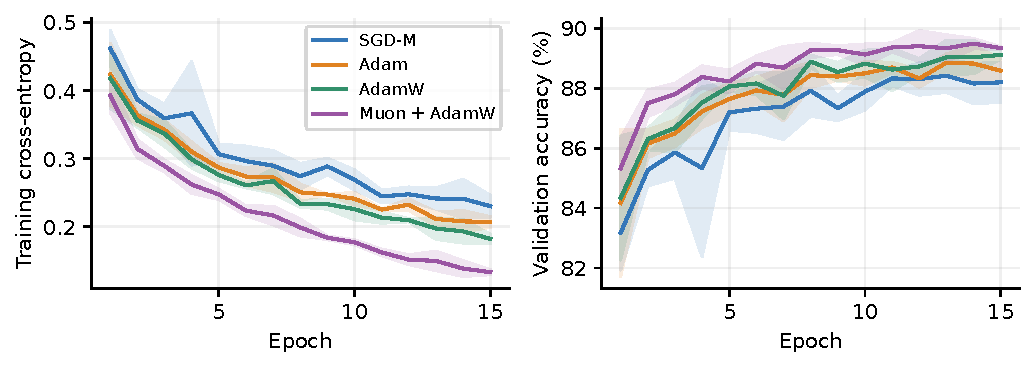
\includegraphics[width=.96\textwidth]{figures/convergence.pdf}
\caption{Training-set loss at epoch-end checkpoints and validation accuracy at equal epochs/updates. Lines are means; bands show one sample standard deviation over three seeds.}\label{fig:convergence}\end{figure*}

\section{Experimental Setup}
\paragraph{Data and pairing.}
Fashion-MNIST \cite{fashion} has 60,000 official training and 10,000 official test examples. We hold out 1,000 training examples per class for validation (split seed 2026), leaving 50,000 for training. Pixels are divided by 255; no statistics are fitted, and there is no augmentation or dropout. Batch size is 128, including the last partial batch: 391 updates per epoch. All configurations for a seed share identical initial weights and batch permutations. The test tensors are loaded only by a separate final-evaluation script, after tuning and all final training are frozen.

\paragraph{Equal tuning budget.}
Each optimizer receives three learning rates and ten epochs per candidate, using development seed 17. SGD tests $\{.01,.03,.1\}$; Adam and AdamW test $\{.0003,.001,.003\}$; Muon tests $\{.005,.02,.05\}$. We select the highest validation accuracy attained, breaking ties by lower validation loss then lower rate. Auxiliary Muon AdamW settings are fixed, so no extra search trials are granted. There is no learning-rate schedule. Selected configurations are independently rerun for 15 epochs (5,865 updates) with seeds 101, 202, and 303. Reported standard deviations use $n-1$ in the denominator. Three seeds quantify run variability only weakly and are not evidence of a universal ranking.

\paragraph{Checkpoints and timing.}
Primary test accuracy uses the validation-best checkpoint; final-epoch accuracy is also reported to preserve the equal-step comparison. A common 85\% validation threshold was specified before tuning. Threshold time is recorded at the first epoch-end observation, without interpolation; a missing crossing is censored, not zero.

Experiments execute sequentially on one NVIDIA H200 (driver 580.105.08), Python 3.12.3, PyTorch 2.11.0+cu130, and CUDA 13.0. Twenty disposable training steps warm each configuration; model, optimizer, and RNG are then recreated. We synchronize CUDA around training and validation. Datasets are GPU-resident. Training time includes minibatch indexing, forward, backward, and all optimizer updates; data loading, warmup, extra train-set evaluation, and checkpoint I/O are excluded. No compilation, autotuning, AMP, or TF32 is used. GPU peak memory is process tensor allocation, including resident data, rather than total device use. Other GPUs retain keep-alive workloads; GPU 0 has no keep-alive competitor. Shared CPU resources and hardware scheduling remain possible noise sources.

\paragraph{Common-time readout.}
After the smoke test and before full-data training, a five-second cumulative \emph{training plus validation} budget was fixed. We select the validation-best completed epoch available by that budget from each trajectory. This is an epoch-boundary retrospective readout, not a separately interrupted end-to-end timed run. Unused time within the next epoch and excluded reporting overhead limit its interpretation as a strict wall-clock comparison.

\begin{table*}[t]\centering
\caption{Measured efficiency. Train seconds exclude validation; threshold seconds include it. Throughput is in thousands of training samples/s. Peak allocated MiB includes GPU-resident development data.}
\label{tab:efficiency}\begin{tabular}{lrrrrr}\toprule
Method & Train (s) & Epoch (s) & k samples/s & Time to 85\% (s) & Peak (MiB)\\\midrule
SGD-M & \pmv{9.40}{0.21} & \pmv{0.63}{0.01} & \pmv{79.83}{1.80} & \pmv{1.43}{0.35} & \pmv{257.0}{0.0}\\
Adam & \pmv{11.31}{0.19} & \pmv{0.75}{0.01} & \pmv{66.31}{1.12} & \pmv{0.99}{0.42} & \pmv{258.3}{0.0}\\
AdamW & \pmv{11.16}{0.08} & \pmv{0.74}{0.01} & \pmv{67.20}{0.51} & \pmv{0.98}{0.43} & \pmv{258.3}{0.0}\\
Muon+AdamW & \pmv{22.04}{0.08} & \pmv{1.47}{0.01} & \pmv{34.03}{0.13} & \pmv{2.02}{1.00} & \pmv{257.8}{0.0}\\
\bottomrule\end{tabular}\end{table*}
\begin{figure*}[t]\centering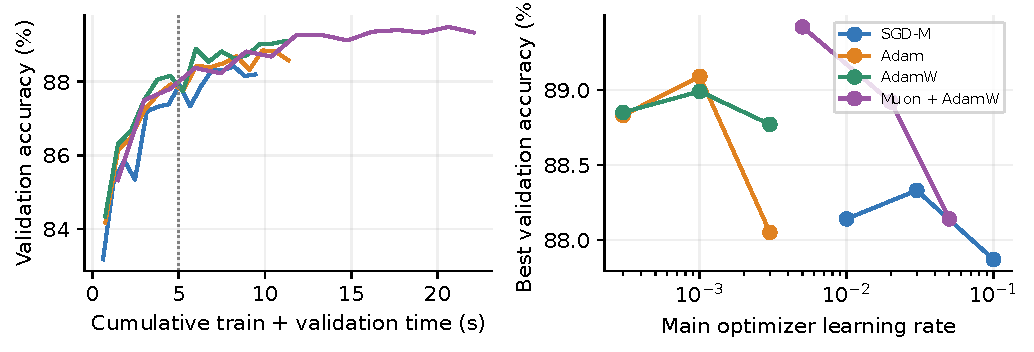
\includegraphics[width=.96\textwidth]{figures/efficiency_sensitivity.pdf}
\caption{Left: validation accuracy against measured cumulative training-plus-validation time; dotted line is the five-second budget. Right: validation-best accuracy for each of three learning-rate candidates (one tuning seed, ten epochs). Muon changes only its matrix learning rate; auxiliary AdamW stays at $10^{-3}$.}\label{fig:time}\end{figure*}

\section{Results and Discussion}
\paragraph{Accuracy and generalization (RQ2).}
Table~\ref{tab:accuracy} reports validation-selected checkpoints. Muon+AdamW has the highest mean test accuracy (\pmv{89.04}{0.29}\%). All values use three seeds, not repeated evaluations of one model. The final-epoch column checks whether checkpoint selection changes the interpretation.


\paragraph{Convergence (RQ1).}
The first observed 85\% validation crossing occurs at mean epochs 2.33 (SGD-M), 1.33 (Adam), 1.33 (AdamW), 1.33 (Muon+AdamW). AdamW is fastest by the corresponding training-plus-validation time. Figure~\ref{fig:convergence} shows that ranking by early progress need not match ranking by the final checkpoint. Epoch-end training loss is evaluated on the full training subset, avoiding the changing-model average implicit in an online minibatch loss.
\paragraph{Computational efficiency (RQ3).}
SGD-M has the lowest 15-epoch training cost. Muon takes 1.97$\times$ AdamW time (22.04 versus 11.16 seconds). The extra matrix operations and auxiliary optimizer calls are plausible causes of the overhead, but epoch timing alone does not attribute cost to individual kernels. All methods have the same samples per epoch; throughput therefore expresses the same cost on a per-sample scale.


At the five-second readout, validation-best-so-far checkpoints achieve test accuracies of \pmv{86.94}{0.52}\% (SGD-M), \pmv{87.21}{0.56}\% (Adam), \pmv{87.54}{0.12}\% (AdamW), \pmv{87.18}{0.57}\% (Muon+AdamW). AdamW has the highest mean under this specific accounted-time budget. The budget selects different training durations; this is complementary to, rather than interchangeable with, the fixed-epoch comparison. A strict online deadline, data-loading cost, or a larger model could alter the ranking.
\paragraph{Learning-rate sensitivity (RQ4).}
Across the three tested rates, the best-validation range spans 0.46 points (SGD-M), 1.04 points (Adam), 0.22 points (AdamW), 1.28 points (Muon+AdamW). This range measures sensitivity within the specified grids, not over all rates. A single tuning seed can favor a configuration by chance; three equal trials do not guarantee equally comprehensive searches for different algorithms. Muon has an additional fixed auxiliary learning rate whose sensitivity is not explored. Its winning main rate, .005, lies at the lower grid boundary, so a better rate outside the grid remains possible.
\paragraph{Interpretation and limitations.}
Muon changes mean test accuracy relative to AdamW by +0.45 points while requiring 1.97$\times$ the training time. Its approximate orthogonalization changes update geometry, but that mechanism alone does not imply a gain on this dataset. Higher training accuracy is not sufficient evidence of better generalization: the train--test gaps in Table~\ref{tab:accuracy} must be read with test accuracy, not minimized in isolation. The gaps compare accuracies at the same checkpoint, not training accuracy averaged during optimization.
The largest confounds are parameter routing (only 39.1\% of parameters use Muon), fixed regularization strength, a short horizon, one dataset, and the small number of seeds. A hybrid-control experiment with identical auxiliary AdamW for every method would help isolate the hidden-matrix optimizer. The current experiment supports configuration-level conclusions only. Muon reaches 94.03\% mean training accuracy with a 4.99-point train--test gap, compared with AdamW at 92.68\% and 4.09 points. The additional fitting transfers only partly to test accuracy. Adam and AdamW cross 85\% validation at nearly the same measured time (0.99 versus 0.98 seconds), far smaller than their seed variation; this is not a meaningful speed separation. Sample SD reflects seed variation on one split and GPU; it excludes uncertainty over data splits, hardware, implementation choices, and hyperparameter search. No statistical significance or general superiority is claimed.


\section{Conclusions}
Under equal ten-epoch tuning trials and a 15-epoch final budget, Muon+AdamW obtains the highest mean validation-selected test accuracy, while SGD-M has the lowest training cost. Muon achieves \pmv{89.04}{0.29}\% test accuracy with an explicitly mixed parameter update scheme. Accuracy per step, accuracy per second, and learning-rate robustness provide different evidence; no single metric justifies choosing an optimizer for every task. Broader datasets, routing controls, and more tuning seeds would be the most useful next checks.


\paragraph{AI usage and reproducibility.}
OpenAI Codex \cite{codex} substantially assisted protocol design, code generation, experiment execution, validation, plots, and drafting. Context7 and web/repository retrieval supported documentation checks. All numerical results come from the saved runs, not generated examples or borrowed measurements. Automated checks do not establish that the student has independently reviewed every claim. The repository includes configuration, source hashes, environment details, raw epoch CSVs, checkpoint evaluation hashes, and the development report. The student remains responsible for understanding and verifying the submission.

\newpage
{\normalsize\bibliographystyle{unsrt}\bibliography{references}}
\clearpage
\onecolumn
\section*{Supplementary Pages: Core Code and Verification}
The following excerpts are taken directly from the runnable source. They explain the optimizer partition, measurement boundary, and test isolation. Third-party optimizer internals are called unchanged through PyTorch. Full scripts and raw results accompany the repository. Each training seed resets model initialization and an independent CPU permutation generator; tests check exact repeatability within this environment, not across hardware or library releases.
\lstset{language=Python,basicstyle=\ttfamily\fontsize{10}{11}\selectfont,
 breaklines=true,columns=fullflexible,keepspaces=true,showstringspaces=false,
 frame=single,rulecolor=\color{black!25},commentstyle=\color{black!65},
 numbers=none,aboveskip=6pt,belowskip=6pt}
\subsection*{S1. Parameter routing and optimizer construction}
Biases receive zero decay. The input and classifier matrices belong to auxiliary AdamW. The two hidden matrices belong exclusively to Muon; explicit identity checks reject overlaps or omissions.
\lstinputlisting{../src/optimizers.py}
\clearpage
\subsection*{S2. Paired initialization, warmup, and measured training}
Warmup updates are discarded. After reseeding, a fresh model and optimizer start the actual run. Training and validation are synchronized separately. Additional train-set evaluation and checkpoint writes are outside the cumulative training-plus-validation clock.
\lstinputlisting{generated_train_excerpt.py}
\clearpage
\subsection*{S3. Evaluation and test isolation}
Evaluation uses inference mode and divides summed loss and correct predictions by the full sample count. No gradients are computed and no test metric is used in model selection. The final evaluator checks a frozen selection manifest, then reads train, validation, and official test splits for predeclared checkpoints.
\lstinputlisting{../src/evaluate.py}
\lstinputlisting{generated_eval_excerpt.py}
\subsection*{S4. Acceptance evidence}
Thirteen optimizer/data/schema/resume unit tests passed. The experiment audit verified 12 tuning runs, 12 formal runs, and 308 epoch rows including eight smoke rows. It checks paired initial-weight hashes, equal tuning budgets, checkpoint hashes, validation-based selections, and mean/sample-SD recomputation from raw data. Core files are available under \texttt{src/}, \texttt{scripts/}, and \texttt{tests/}. Run \texttt{python scripts/validate\_results.py} after evaluation and plotting.

\end{document}
